\section{A 150 years perspective on society, economy and technology}


\paragraph{Five distinct time periods}

\begin{enumerate}
    \item The 'Gilded Age' from 1870 until 1910
    \item The 'First Shift' from 1911 until 1946
    \item The 'Golden Age' from 1947 until 1968
    \item The 'Second shift' from 1969 until 1979
    \item The 'Fool's Gold Age' from 1980 until 2008-2019
    \item The 'Third Shift' from 2019 to \dots
\end{enumerate}

\paragraph{Three ages}
Three structural regimes clearly stand out because of their specific
characteristics and their very different growth drivers, we will call them:
\begin{itemize}
    \item \underline{Gilded}: Covering thinly with gold leaf or gold paint
    \item \underline{Golden}: Made or consisting of gold, very happy and prosperous
    \item \underline{Fool's Gold}: Pyrite's metallic luster and pale brass-yellow
        hue give it a superficial resemplance to gold, hence the well-known
        nickname of fool's gold
\end{itemize}

\paragraph{Shifts}
\begin{itemize}
    \item When one structural economic regime passes into another, the
        economic system goes through a shift.
    \item Because each shift experiences the end of one era and the
        beginning of another, it always comes with geopolitical,
        financial and economic disruption and distress.
    \item However, during these shifts, also reforms takes place, where
        the seeds are planted from which a new structural regime takes
        root.
\end{itemize}

\subsection{The Gilded Age (1870 - 1910)}

\begin{itemize}
    \item Era of rapid expansion of heavy industries and infrastructure
    \item Accelerated innovation from the Technological Revolution let to
        interconnected growth: Telegraphs, railroads, transatlantic ship
        routes
    \item First wave of globalization: Rise of the 'haute finance',
        centered around the Gold Standard, with the British Pound as
        reserve currency
    \item The stock market, during those decades, was solid, with high
        earnings qualities and a strong underlying economic growth
    \item The balance of power, between the newly created nation states,
        guaranteed geopolitical stability. This prevented the occurence
        of any long and devastating war between the Great Powers. In France,
        this epoch was called the 'Belle Epoque'.
\end{itemize}

\paragraph{Colonialism rising to its peak}
The combined populations of the Western European colonial powers were
roughly 200 million at that time whereas more than 800 million people
were living in the colonies. WW2 curtailed what was left of Western
European imperial ambitions and the US, forming by itself a whole
continent enjoying access to a protection from two oceans, became the new
geopolitical behemoth. The end of colonialism came with the rise of the US
as an empire, and the end of Western European imperial ambitions.

\paragraph{The first wave of globalization}
Infrastructure was comparable to now. You could order things on the phone
and travel with and without passports. There was also a certain amount
of wealth.

\vspace{1\baselineskip}

Inequalities were at a historical high:
\begin{itemize}
    \item Urbanization and migration led to an oversupply of labor in the
        cities
    \item a stagnation of real wages
    \item and a decline of the proportion of GDP goint to labor
\end{itemize}
Robber baron capitalism and winner-takes-all markets created monopolies.
So the fruits of progress stayed in the hands of the happy few.

\vspace{1\baselineskip}

There was a high urbanization and migration.

\vspace{1\baselineskip}

A period of wild financial and economic expansion with a lack of
institutions and regulations to smoothen boom and fight bust. As a result
we see multiple cycles of boom $\rightarrow$ panic $\rightarrow$ depression.

\begin{itemize}
    \item $8$ years of overinvestment and speculation, and a railroad
        boom after the end of the american Civil War (1865) ended in the
        panic of 1873.
    \item This was followed by the Long Depression wihch lasted until 1879
    \item A new boom started pushed by the Technological Revolution, this
        lasted until the panic of 1893
    \item Ensued by another depression which lasted until 1897
    \item Followed by another boom, which ended in a massive banking crisis
        in 1907. 
\end{itemize}

The Gold standard:
\begin{itemize}
    \item Money is linked to gold, so the standard unit of account in the
        economy is gold.
    \item Because of this, it becomes difficult for countries to 'create
        money' a.k.a. to 'expand the money supply to stimulate the economy'
    \item It was adopted internationally, so capital could flow freely from
        one country to another, and you could always exchange your currency
        for gold, so this was a serious protection for owners of capital.
\end{itemize}

Nations that adopted the gold standard were forced to manage capital flows
instead of employment:
\begin{itemize}
    \item When there was a recession, governments increased interest rates
        to stop the outflow of capital (and gold).
    \item Because the crisis could not be countered with expansionary
        monetary policies, the economy contracted.
    \item Less demand in labor and in goods, would make prices drop.
    \item The supply of cheaper products would make a country more
        competitive on the global markets. This would restore the external
        balance and would attract a renewed inflow of capital (and gold)
        - a kind of negative feedback system.
    \item Gold convertibility (and fixed exchange rates) protected capital
        at the expense of labor. Thsi resulted in dramatic decline in wages,
        rise in unemployment and a sharp rise in business and bank failures
        during times of crisis.
\end{itemize}

If a nation's economy were a human body, then its heart would be the central
bank. And just as the heart works to pump life-giving blood through the
body, the central bank pumps money in the economy to keep it healthy and
growing. Sometimes economies need less money, and sometimes they need more.

At the micro-level, easy access to money means more spending, investment and
consumption by people and by businesses.

\pagebreak

\subsubsection{The trilemma of international finance}

\begin{minipage}{0.55\textwidth}
    Economic policy makers want to achieve three goals:
    \begin{itemize}
        \item Open their country's economy to international flows of capital
            or to bring in foreign capital and to allow the nation's citizens
            to diversify their investments abroad.
        \item Follow an independent monetary policy to stabilize their economy
            and support employment and support employment in times of need.
        \item Have a fixed foreign exchange rate which brings stability and
            trust in international trade and investment.
    \end{itemize}
\end{minipage}
\hspace{10pt}
\begin{minipage}{0.4\textwidth}
    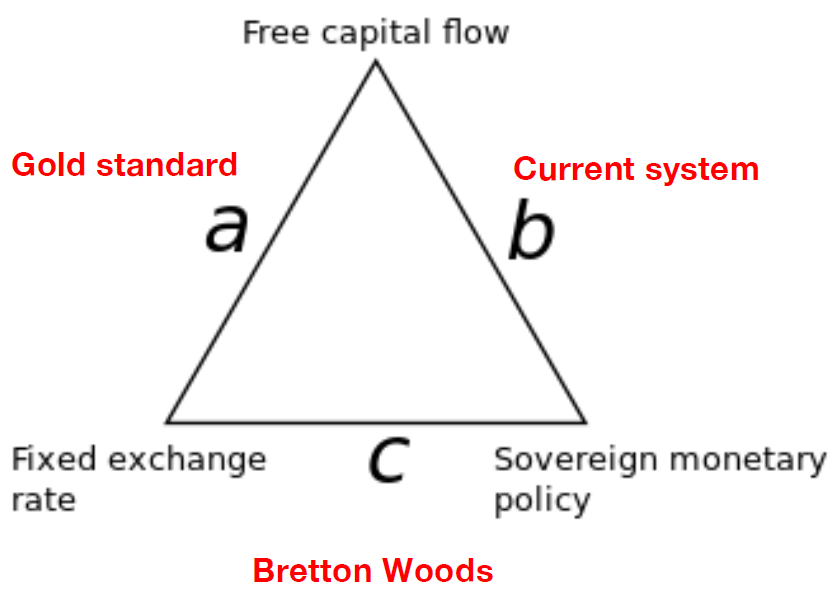
\includegraphics[width=\textwidth]{Pictures/trilemma.png}
\end{minipage}

\vspace{1\baselineskip}

Suppose a government wants to fight a recession by cutting its interest rates.
If capital can flow freely, this will result in a net outflow of capital in
search for a higher yield. This outflow will depreciate the currency - so you
cannot have a fixed exchange rate. Vice versa: If a government wants to fight
inflation by increasing its interest rates. If capital can flow freely, this
will result in a net inflow of capital in search for higher yield. This will
increase the value of the currency. You can only have two out of three:

\begin{itemize}
    \item \underline{Gilded Age}: Fix exchange rate and let money freely
        across the globe at the loss of an independent monetary policy.
    \item \underline{Golden Age}: Fix exchange rate and follow independent
        monetary policy at the loss of free capital flows.
    \item \underline{Fool's Gold Age}: Follow independent monetary policy and
        let money flow freely across the globe at the expense of a fixed
        exchange rate.
\end{itemize}

Bretton Woods is fully top-down steered, Gold Standard is fully bottom-up
laissez-faire, the current system is in the middle.

\subsubsection{Shifts}

\begin{itemize}
    \item When one structural economic regime passes into another, the economic
        system goes through a shift.
    \item Because each shift experiences the end of one era and the beginning
        of another, it always comes with geopolitical, financial and economic
        disruption and distress.
    \item However, during these shifts, also reform takes place, where the
        seeds are planted from which a new structural regime takes root.
\end{itemize}


\subsection{The First Shift (1911 - 1946)}

The first shift was characterised by nationalism, imperialism, war,
revolution, depression and genocide. There was huge unemployment.

\vspace{1\baselineskip}

Institutional reform with Roosevelt' New Deal (1933-1939):
\begin{itemize}
    \item \underline{Stabilizing the banking system} through bank reform acts
        (e.g. Glass-Steagall, establishment of the Federal Deposit Insurance
        Corporation - FDIC)
    \item \underline{Suspension of the Gold Standard}, with a freely floating
        US Dollar and increase of money in circulation by the Federal Reserve
    \item Increase \underline{transparency in the stock market} by mandatory
        publication of balance sheet, profit and loss statement\dots
    \item \underline{Public works and relief}: Hire unemployed to build schools,
        municipal buildings, waterworks, sewers, streets, parks airports, hospitals\dots
        (Civil Works / Public Works Administration)
    \item \underline{Social security act} establishing a permanent system of
        pensions, unemployment insurance, welfare benefits\dots
    \item \underline{National Labor Relations Act} guaranteed workers the
        right to collective bargaining through unions
    \item \underline{Fair Labor Standard Act} set maximum of 44 hours of work
        per week and minimum wages, child labor under 16 was forbidden
    \item \underline{Wealth Tax Act}: redistribute wealth by imposing a tax
        of 79\% on income over 5 million USD.
\end{itemize}

Wartime stimulus and massive capital investment during WW2:
\begin{itemize}
    \item The number of machine tools in the US doubled between 1940 and 1945.
    \item Almost all of these were paid for by the government.
    \item Because all were state-of-the-art, they could be reconverted to produce
        consumer goods after the war.
\end{itemize}

High-pressure economy of WW2 with 'infinite demand', created an environment
of 'Learning by doing' where everybody on all levels was eager to increase
efficiency and reduce costs. This working culture, adopted during the wartime
period, and the best-practices resulting from it, persisted after the war had
ended. As an example, in 1942, it took 8 months to build a standard Liberty
freighter ship, by the next year, this had been reduced to a few weeks.

\subsubsection{Bretton Woods}

In the summer of 1944 (3 weeks after D-day), 730 representatives of 44
countries gathered at the Bretton Woods conference with the ambitious goal
to redesign the international monetary system, the new system should:

\begin{itemize}
    \item replace the monetary chaos of the interwar period with a new
        international system that would support trade through stable exchange
        rates.
    \item Free trade was preferred to free capital flows, expecially to
        short-term 'hot money' flows and capital flight, and as such, it was
        explicitly recognized that countries needed to impose capital controls.
    \item Each country could still follow an independent monetary policy to
        fight recessions and stimulate employment.
\end{itemize}

Lessons would be learned from the past, and, more specifically from the
mistakes that had been made in the interbellum period where countries had
re-joined and then abandoned the gold standard following a beggar-thy-neighbour
strategy in a series of competitive devaluations. Protectionism had risen and
economic cooperation between the great powers had vanished leading to a
deepening and lengthening of the Gread Depression, which pushed many countries
into totalitarianism.

\vspace{1\baselineskip}

After the war, the idea rose to support trade through international cooperation,
but still be able to fight recessions with independent monetary policy. This
imposed capital controls.

\vspace{1\baselineskip}

After the war, "the Greenback was the only currency left standing and capable
of lubricating world trade".

\vspace{1\baselineskip}

Bretton woods established a system of payments based on the dollar, which
defined all currencies in relation to the dollar, itself convertible into
golt, and above all "as good as gold" for trade. US currency was now
effectively the world currency, the standard to which every other currency
was pegged.

\paragraph{Back to the trilemma of international finance}
The current system has the advantage that exchange rates can buffer an
economic shock, when a currency devalues, exports from that country become
very cheap. This is an alternative to devaluation through wage decreases.
However, free flow of capital creates flows of 'hot money'\dots see crises
of 1994 and 1997.

\paragraph{Lessons learned}

From the calamities during the first shift, lessons were learned from which
the Golden Age would rise:

\begin{itemize}
    \item Institutions were reformed \underline{to fight the Great Depression}.
    \item A social welfare system was installed \underline{to counter the
        upcoming Bolshevik revolution}.
    \item \underline{WW2} let to massive stimulus and capital investment.
    \item \underline{To fight nationalism}, and support trade in a balanced
        way, the international financial system of Bretton Woods was set up.
\end{itemize}


\subsection{The Golden Age (1947 - 1968)}

The two decades after WW2 were blessed with extraordinary economic growth:
\begin{itemize}
    \item Mean reversion: Recovery of the economy to its full potential
        after WW2.
    \item Stimulus: reconstruction of infrastructure and industry
    \item Productivity increase from technical innovations and capital
        investments
\end{itemize}

A social contract between workers and owners on
\begin{itemize}
    \item The parallel growth of real wages and productivity
    \item ensuring that the fruits of the economic progress were equitably
        shared
    \item Led to wealth accumulation and spare time $\Rightarrow$ CONSUMERISM
\end{itemize}

\paragraph{Inequality from the stone age to the 21st century}

"Thousands of years of history boil down to a simple truth: ever since the
dawn of civilization, ongoing advances in economic capacity and state
building favoured growing inequality but did little if anything to bring
it under control." Inequality will always have the natural tendency to increase,
only violent ruptures have been able to flatten it:

\begin{itemize}
    \item Mass mobilization warfare
    \item Transformative revolution
    \item State failure
    \item Lethal pandemics
\end{itemize}

\paragraph{Consumer Society}
Free time and wealth accumulation created a consumer society with new demand
for consumer goods like electrical apparel, automobiles or entertainment
services.

\paragraph{The Rise of hydrocarbon man}
During the Gilded Age, coal has been the primary energy source. During the
Golden Age, Oil and Natural Gas have been added to mix and taken up a bigger
proportion. The West becape very much dependent on fossil fuels.

\paragraph{The Fall}

"The Great Society rests on abundance and liberty for all. It demands an end
to poverty and racial injustice\dots The Great Society is a place where every
child can find knowledge to enrich his mind and to enlarge his talents\dots
It is a place where the city of man serves not only the needs of the body and
the demands of commerce but the desire for beauty and the hunger for cummunity."
changed to "Things fall apart, the center cannot hold. Mere anarchy is loosed
upon the world\dots" Anarchy and countercultures emerged.


\subsection{The Second Shift (1969 - 1979)}

\paragraph{The Nixon shock and the end of Bretton Woods (1971)}

\begin{itemize}
    \item The Bretton Woods system was based on trust in the US Dollar.
    \item But the US overstreched in a Vietnam war combined with rising
        public expenditures in the Great Society programs
    \item At a certain point there were more dollars in the hand of foreign
        countries (so-called eurodollars) then the total gold stock of the US
    \item Trust in the US Dollar, which was the keystone of the Bretton Woods
        system, evaporated
    \item In February 1965, President Charles de Gaulle sent the French Navy
        across the Atlantic to pick up the French reserve of gold, a gesture
        which was soon followed by other countries.
\end{itemize}
As long as the US had a trade surplus, all the dollars it was sending out,
came back. When reversed, the Eurodollar pool became a lake and a sea. The
world was awash with dollars that were all supposed to be backed by Gold.

\begin{itemize}
    \item The US gold reserves, which were at 65\% of the world monetary stock
        in 1952, reduced to 29\% in 1967, 15 later.
    \item The opposite happened in Europe, where the combined gold reserves
        of France, Germany and the UK were at 6\% of global stock in 1952,
        increasing to 26\% in 1967.
    \item This dynamic ended on August 15, 1971, with the 'Nixon Shock', when
        the US President Richard Nixon unilaterally ended the convertibility
        of the Dollar to gold. This was the end of the Bretton Woods system.
\end{itemize}

\paragraph{Peak Consumption}
You can only buy a limited amound of stuff, technology adoption follows
the S-shape of the logistic growth process, where the strongest growth
rate can be observed during the Golden Age.

\vspace{1\baselineskip}

Economic paradigm shift from falling unemployment with rising inflation,
to stagflation. Fiscal and monetary overstreching because of Lyndon Johnson's
Great Society and the Vietnam war.

\paragraph{Philips' Relation}
Intuition: A falling unemployment rate signals an increase in the demand
for labor, which puts upward pressure on wages. Profit-maximizing firms then
raise the price of their products in response to rising labor costs.

\vspace{1\baselineskip}

From the end of the fifties, throughout the sixties, many economists were
convinced that there was a fundamental and permanent relationship between
inflation and unemployment. It was conjectured that the process underlying
this 'law of nature' was based on a virtuous cycle where higher demand for
goods would increase prices, which in turn would encourage companies to hire
more personal, increasing general employment, and again driving up demand
in a positive feedback loop. This relationship, called the \fat{Phillips
curve}, was one of the empirical backbones of Keynesian policy. It was believed
that governments could make a trade-off between inflation and employment.
Government spending and tax reductions could be used to stimulate the economy,
which would have inflationary effects. However, a reasonably high level of
inflation would be acceptable as this would lead to a lower unemployment through
the Phillips relationship. As such, it was believed that governments could
spend their way out of a recession by cutting taxes and boosting government
spending. Any inflation that would come as a by-product of this policy would
be politically acceptable as it would result in higher employment through
the Phillips curve.

\vspace{1\baselineskip}

In the beginning of the 1970s, western countries started losing their grip
on oil exploitation, this let to 2 oil shocks:
\begin{itemize}
    \item Firs oil shock with the OPEC oil embargo as a reaction to the
        Yom Kippur war (1973 Arab-Israel war)
    \item Second oil shock with the Iranian revolution under the leadership
        of Ayatollah Khomeini (December 1978 / January 1979)
\end{itemize}

The most dramatic knock-on effect that would lead to the first oil shock and
as such would contribute to the global power shift in oil markets, came about
in October 1973, when a coalition of Arab forces, led by Egypt and Syria
launched a surprise attack on Israel on the Jewish holy day of Yum Kippur,
the Day of Atonement. The Yum Kippur war lasted only three weeks, featured by
intense fighting with one of the most spectacular reversals in military
history, when the Israelis managed to turn around a hopeless situation 'from
being within hours of extinction to shattering the invadeing forces and advancing
on Damascus and Cairo'. The fact that the Americans had supported the Israeli
forces with military supplies, in a very plain and unsophisticated fashion, at
crucial stages during the three-week period of hostilities, bonded the alliances
within OPEC.


\subsection{The Fool's Gold Age (1980 - \dots)}

\paragraph{The Illusion of the Perpetual Money Machine}

\begin{itemize}
    \item Consumption, not funded by savings but by debt, and by wealth
        extracted from the stock and the housing market
    \item Economic growth, not driven by productivity increase in the real
        economy, but by growth of the financial sector
    \item Further supported by a climate of deregulation and a massive
        growth in financial derivatives
    \item Resulting in a succession of bubbles and crashes, feeding upon
        each other and culminating in the GFC (Global Financial Crisis) of
        2008
\end{itemize}

The ultimate financialization offered by ETFs opens the road to more
bubbles created by the herding mechanism of small investors as well
as large hedge funds and sovereign funds crowding in and out of the
investment fashion of the moment.

\paragraph{Reaganomics / Thatcherism}

\begin{itemize}
    \item Decline in Representation: Decline in Union Membership
    \item Reagen decreased taxes of the rich to provide an incentive to
        save. This would increase investment and create jobs.
    \item The savings of the rich would 'trickle down' to the masses.
\end{itemize}

The sharp rebound in inequality in the US was mainly the result of a shift in
economic policy often referred to as 'Reagonomics' or 'Thatcherism'. John
Komlos, Professor Emeritus at the University of Munich, describes the ideology
of that time as follows: In short, Reagen advocated decreasing the taxes
of the deserving rich, which would provide incentives to increase savings
and investment and thereby create jobs and subsequently 'trickle down' to
the masses so they will benefit from it in due course. Moreover, lower taxes
meant an increase in take-home pay and that would provide an incentive for
people to work harder and for entrepreneurs to take more risk, thereby growing
the economy and boosting incomes.

\begin{itemize}
    \item The fruits of economic growth not equitably shared
\end{itemize}

Method was a bit counterproductive. The rich got ver richer and the poor
only got a little bit richer. The gap increased.

\paragraph{Decreasing Savings, increasing consumption based on debt}

Consumption was paid with debt.

\paragraph{Stock Markets}

The Fool's Gold Age was characterized by a very strong stock market
performance, with lagging earnings. This strong stock market performance
is not reflected in an increase in productivity. To the contrary we see
a secular decline in the productivity in the West over the past 50 years.

\paragraph{Economic Growth}

There is a different picture for China. China paints a completely different
picture with a very strong increase in per capita real GDP over the past 40
years.

\subsubsection{Three waves of globalization}

Globalization is not an inevitable process, and it is also not a linear
process.

\begin{figure}[h]
    \centering
    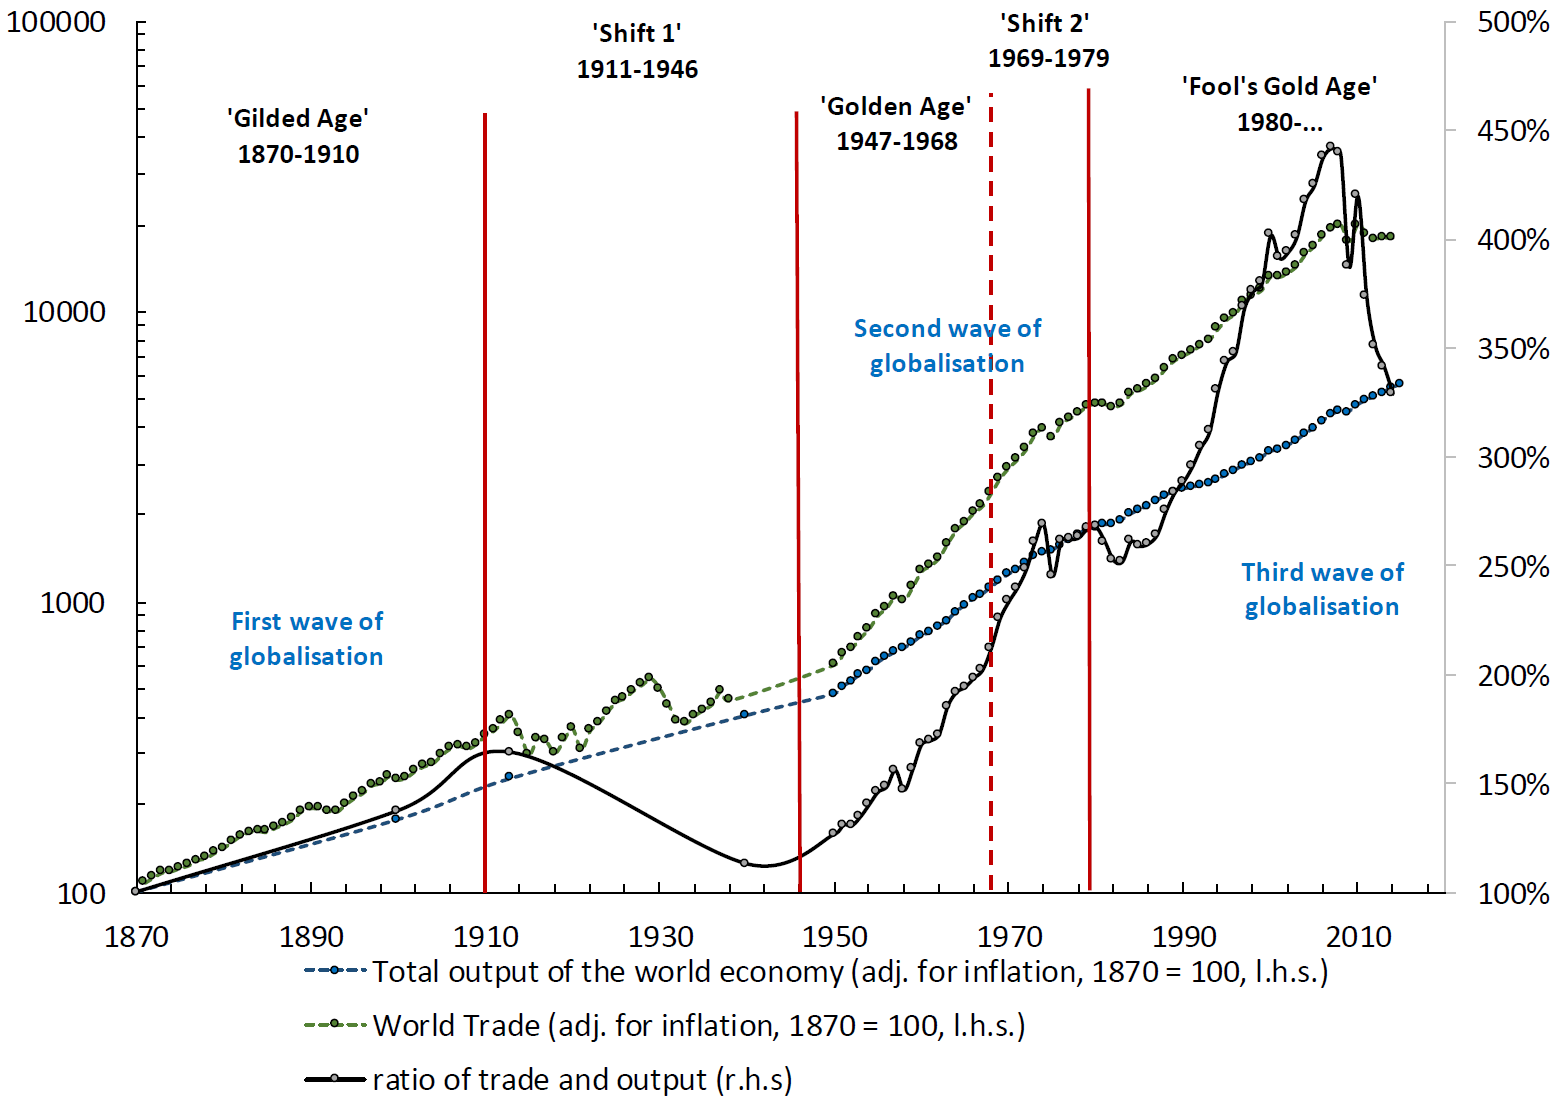
\includegraphics[width=0.6\textwidth]{Pictures/three_waves_of_globalization.png}
\end{figure}

\begin{itemize}
    \item The first wave came with the technological revolution, pushed
        forward by increasing connectivity, falling transportation costs
        and the gold standard and the Pound Sterling that create a global
        marketplace.
    \item The second wave: Renewed international cooperation and trade
        liberalization after nationalism during the First Shift brought
        globalization back to its previous level. But flows between
        emerging and developed markets were limited to those primary
        commodities that did not compete with agriculture in the developed
        countries.
    \item In the third wave, new information and communication systems made
        it possible to manage and control geographically dispersed supply
        chains. Production flowing to places with lower cost of labor.
\end{itemize}

\paragraph{The second vs third wave of globalization}

\begin{itemize}
    \item In the second wave of globalization, resources were extracted
        from developing countries. Trade flows were mainly raw materials
        from developing to developed countries.
    \item In the third wave, developing countries were integrated in the
        global supply chains.
    \item The second wave mainly favored the rich countries. During the
        third wave developing countries made a spectacular catch-up movement.
\end{itemize}

\paragraph{The Economic center of gravity is moving East}

The Economic gravity an dlight mean centre moved to the east.

\paragraph{Debt, Investment, Financialization and Consumption in the Fool's Gold Age}

\paragraph{Debt}

Another characteristic of the Fool's Gold Age is the massive increase
in debt, but the remarkable decrease in the 'efficiency of debt'.
Now one dollar in the non-financial sector 'generates' $25$ cents in
GDP. Student loans and Car loans increased immensly.

\paragraph{Investment}

But this increasing in debt is not used to increase investment in tangible
assets.

\paragraph{Consumption}

Consumption has still increased since the Golden Age, but the mix has shifted
from goods to services (healthcare, pension, financial services, insurance)

\paragraph{Financialization}

Massive growth of the derivatives market up to a current level of $600-700$
trillion USD.
Rise of machines: automatic trading / high-frequency-trading.

\begin{itemize}
    \item Put simple, ETF's are funds that are traded on the stock market
        (ETF = Exchange Traded Funds).
    \item ETFs can specialize in certain investments e.g. gold, or oil,
        or other commodities.
    \item They provide a very easy access for smaller investors to specific
        products, or stategies.
    \item There are now 5 Trillion USD in ETFs outstanding.
    \item Massive growth of the ETF industry.
\end{itemize}


\subsubsection{ETF impact example: Negative oil prices}

What are oil futures?
\begin{itemize}
    \item Futures are standardized contracts between a seller and a buyer
        for the delivery (of oil) at a specific time in the future.
    \item There are future contracts for each month in the future up to
        many years ahead, but the further out the less liquid the
        contract becomes.
    \item Each future contract has its own price evolution, normally,
        the correlation between the contracts will be high, but there
        may be substantial differences nevertheless.
    \item Producers and big consumers of oil use futures contracts to lock
        in a future price to buy or sell the product that they need
    \item If you want to invest (speculate) in the oil (commodities) market,
        you cannot accept physically delivery of the product, then you have
        to buy a future contract.
    \item A graph representing prices as a function of the delivery date
        (x-axis) is called the term structure
    \item If the graph is upward sloping, it is said that the market is
        'in contango'
    \item If the graph is down sloping, it is said that the market is 'in
        backwardation'
    \item If you buy one of these futures contracts, you are obliged to buy
        1000 barrels of WTI Crude Oil at the contract/delivery date.
    \item If you cannot accept this physical delivery, you have to 'sell'
        your contract in time before the settlement date.
    \item This can be at any price, and, as we have seen on April 21 2020,
        even negative prices.
    \item Longer term investors always sell the futures contract before
        the settlement date and use the proceeds to enter a new contract.
        If the market is in contango this results in a loss, if the market
        is in a backwardation it results in a profit.
    \item This is called 'rolling'
\end{itemize}

\begin{figure}[h]
    \centering
    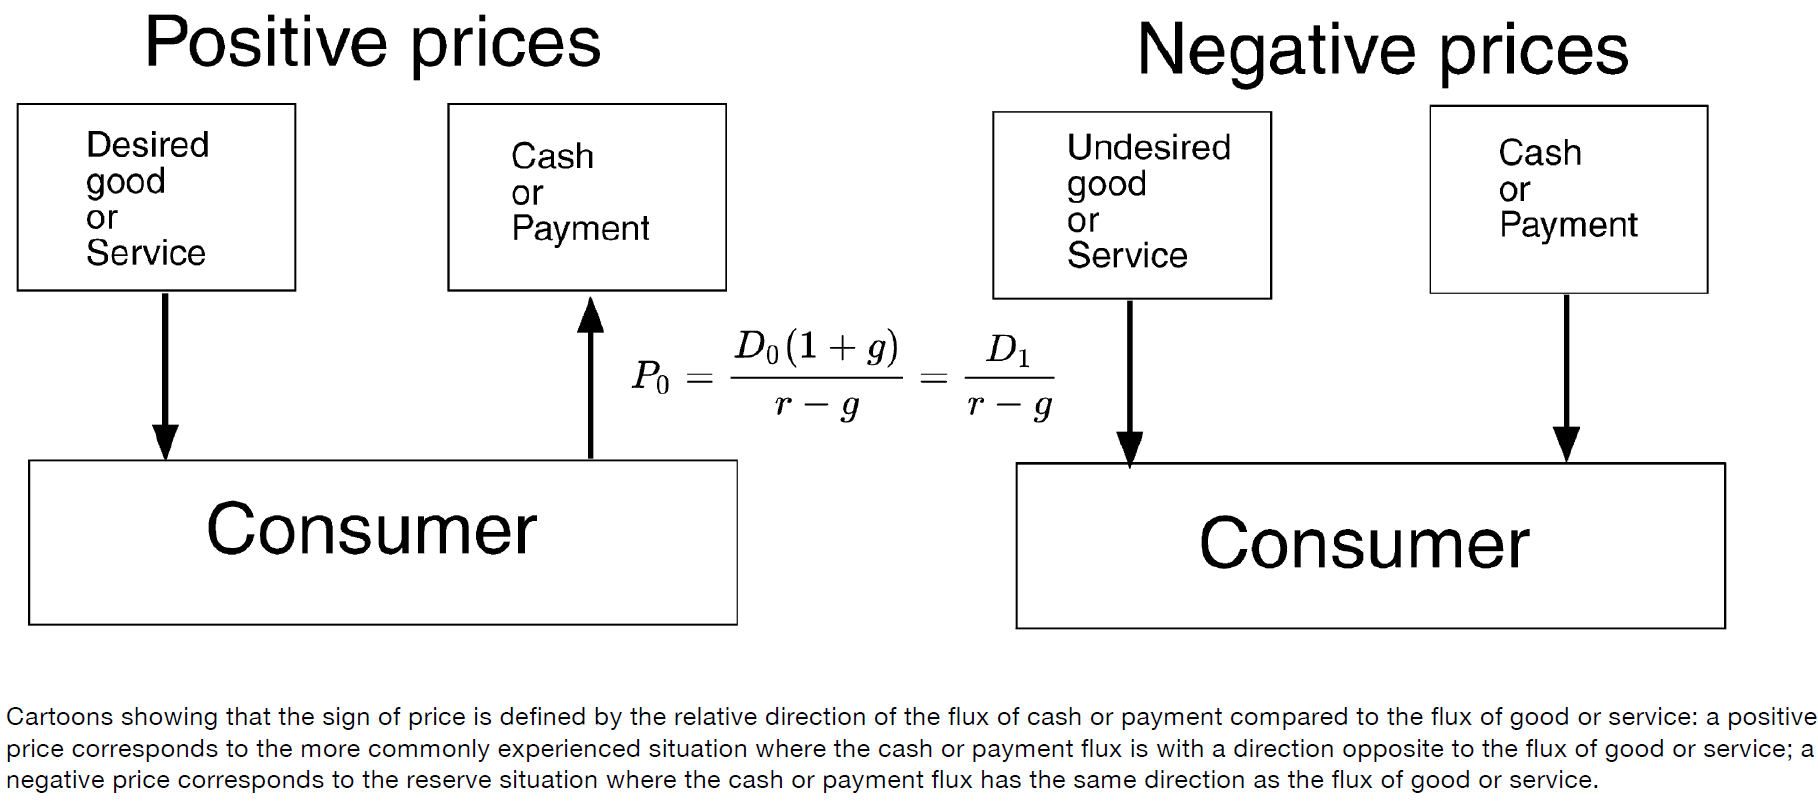
\includegraphics[width=0.9\textwidth]{Pictures/Price_sign.png}
    \caption{Price sign}
\end{figure}

\begin{itemize}
    \item For retail investors, future are not very convention because
        you need to buy 1000 units in one contract.
    \item That is where ETFs come in handy.
    \item Those are stock listed companies that e.g. for oil only buy oil
        futures. You can buy a share in that company on the market e.g. for
        the ETF USO (US oil) you can buy shares at the price of a few USD
    \item An ETF like USO does not want physical delivery and has to roll
        its positions before the settlement date.
    \item With the existing super-contango in oil, this resulted in a monthly
        loss of $33\%$ at the end of April 2020
    \item Over the month of April $2020$ there has been outsized inflow
        (3 Bn USD) in the United States Oil Fund (ETF)
    \item The fund has to roll its future every month and even publishes its
        "roll dates" (when it is selling the near month contract and buying
        the next month contract)
    \item So, between 7/04 and 13/04, 2020, USO had to 'roll' 4 Bn USD of
        oil futures from the front contract to the next.
    \item With this size, USO totally dominated the market of the front
        (selling) and the next month (buying) futures
    \item Because the flows of USO were predictable, many 'professional
        investors' did front running on the ETF
    \item Frontrunning means that they took a position ahead of a large order,
        taking profit from the market impact of that order.
    \item They knew that the front contract would go down, and the next
        contract would go up (relative to each other), so they shorted
        the front and went long the next.
    \item This massive short position on the front contracts hat to be
        closed before April 21. But there were only sellers and no buyers,
        this resulted in a price drop of $-300\%$ on April 20.
    \item The market hat to go in negative territory ($-40$ USD) to find
        "buyers" of the front WTI future contract.
    \item Negative prices were only seen in the front contract. For example,
        if you look at the 6M ahead contract of OCT 2020, you could see a
        large drop from 31 to 25, which is a $20\%$ drawdrop on the same
        day (but not a $300\%$ crash).
\end{itemize}

\paragraph{Bubbles feeding upuon each other in the Fool's Gold Age}

Examples: Black Monday (October 19th 1987), Dotcom Bubble (March 2000),
House price bubble peaking mid-2006

\vspace{1\baselineskip}

The historical evolution of the S\&P500 Index showing the price growing faster
than an exponential up to its tipping pint of 19th October 1987. The dotted
and solid smooth black lines are the results of our model calculations with
two different levels of nonlinearity. Reproduced from the book "Why stock
markets crash" by D. Sornette

\vspace{1\baselineskip}

Quaterly average House Price Index in the 21 states and in the District
of Columbia (DC) where Zhou and Sornette diagnosed bubble-type behaviours in
June 2005 and predicted a peak in mid-2006. For comparison, the HPI has
been normalized to 100 at the second quarter of 1992.

\vspace{1\baselineskip}

US real house prices between 1974 and 2014. Threee peaks in the growth
rate are immediately followed by a correction. When the growth rate itself
grows, the process becomes unstable and a correction follows around the
critical point embedded in the faster-than-exponential growth process.

\subsubsection{Bubble of everything 2007}

\paragraph{Stocks}
The historical evolution of the S\&P500 index shown as dots. The
dashed vertical line shows the last observation used to calibrate our model.
The colored curves show different fits. It is expected that the correction
occurs with 80\% probability in late 2006. This indeed happened.

\paragraph{Oil}
Also crashed mid-2008.

\paragraph{Debt} Bubble also burst.

\paragraph{Globalization Bubble}

The time series represent a proximity index of emerging markets equities
and currencies, freight prices, soft commodities, base and precious metals
and energy.

\subsubsection{Central bank policies as slaves to the stock market}

Federal fund rates are consistently cut after stocks decline. Do central
banks have an unofficial mandate to support stock markets?
The key question, however, is this: did it lead of lag? According to common
wisdom and standard textbook arguments, a decrease of interest rates is
supposed to make borrowing cheaper. This results in increasing expectations
of future growth. Additionally, lower rates mean lower discount factors.
The combined effect should be a boost on stock prices. In this line of
reasoning, a federal funds rate decrease should lead economic growth and
cause stock market prices to increase. This, anti-correlation and a lead
of the Fed rate are expected.

\paragraph{"Primum non nocere" vs the illusion of control}

In the US, there is a zero-tolerance, with the objective to stop all fires.
In Mexico, there is a laissez-faire policy, arguably due to weaker resources
and smaller loss exposure. The results are drastically different: while
Southern California has few small fires, extremely large fires are shockingly
frequent; In contrast, Baja California is graced with many small and essentially
no large fires.

In order for the system to be resilient against catastrophic events, deadwood
needs to be cleared in a natural, dynamic, self-organized way. Could this
observation also be true for the economy? With the special actions that
central banks have been carrying out since the crisis, are we not piling up
deadwood, with the zero-tolerance practice?

\begin{figure}[h]
    \centering
    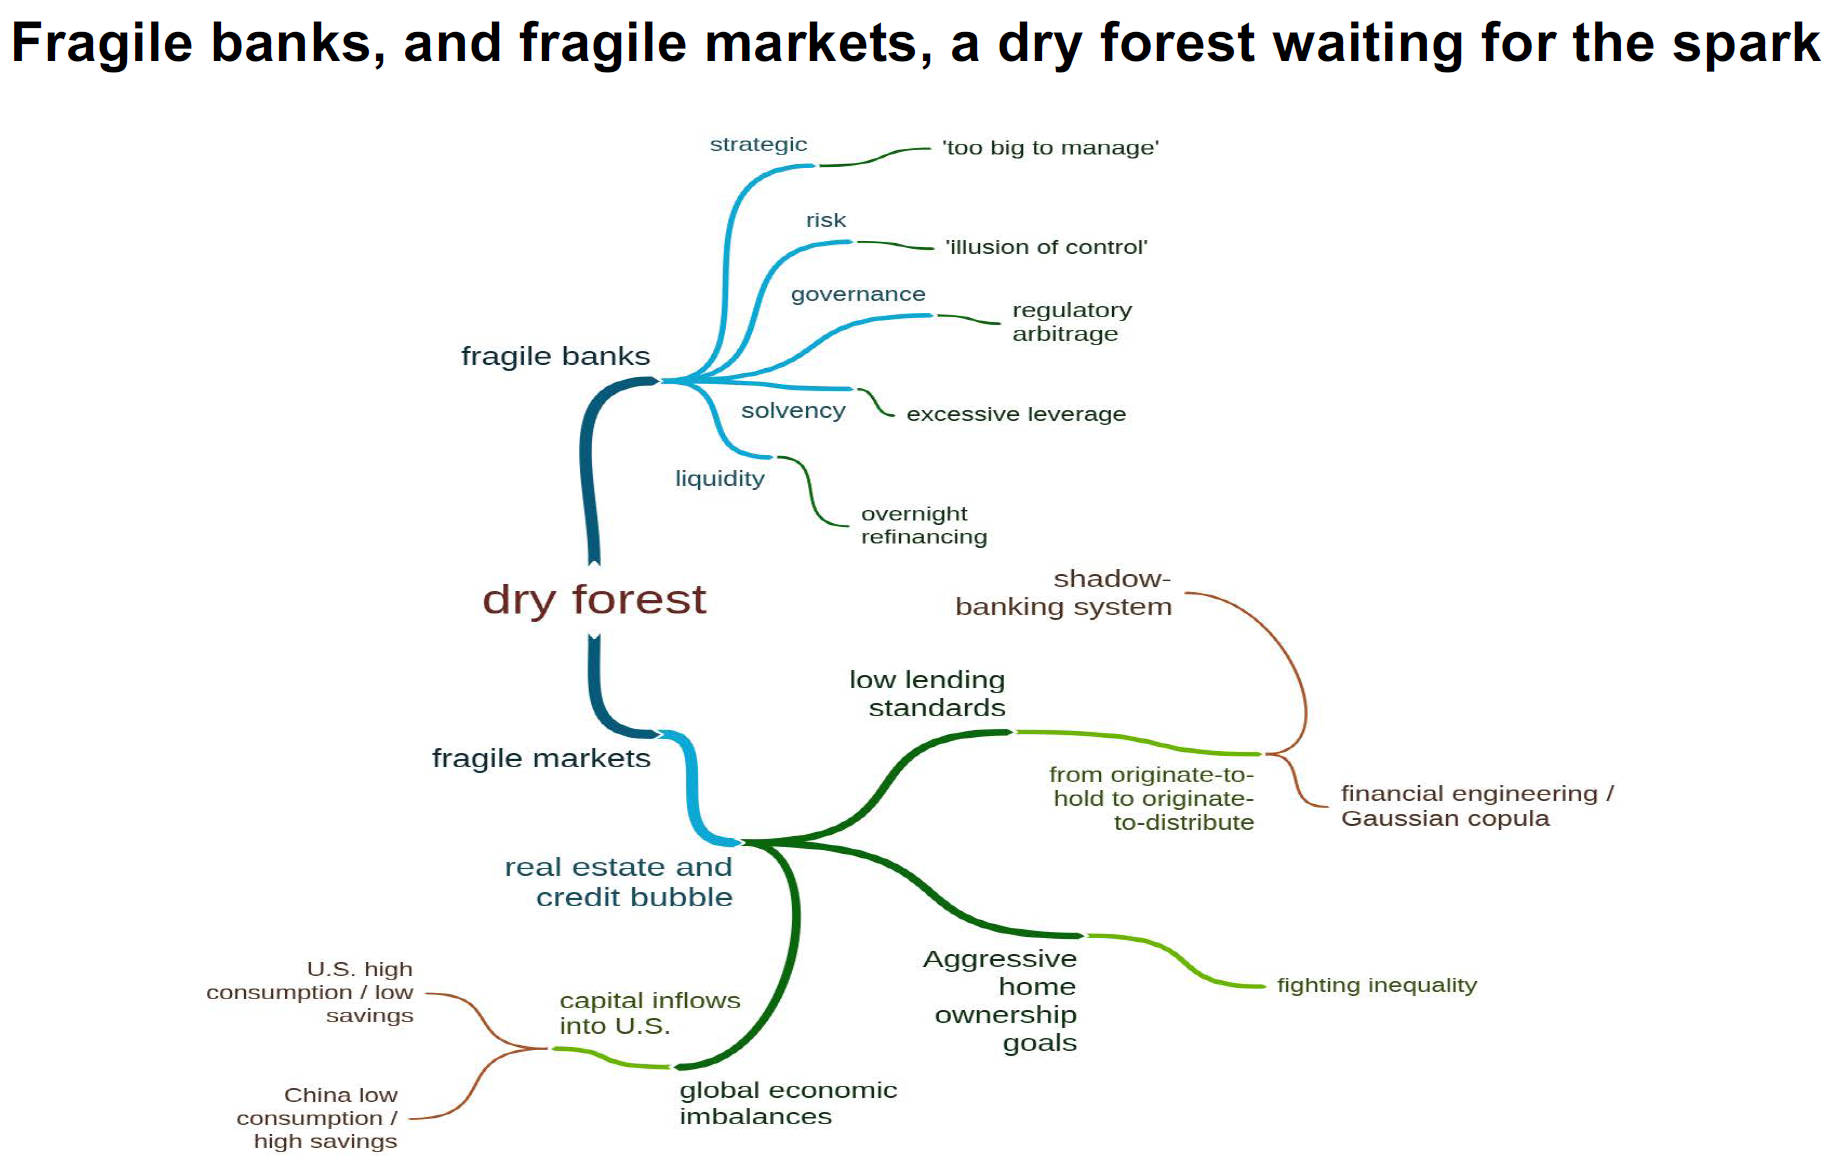
\includegraphics[width=\textwidth]{Pictures/dry_forest.png}
\end{figure}

\subsection{Conclusion}

\paragraph{The super-business cycle - a 150 year endogenous view on
economy and society}

We have described the three economic regimes and the two shifts of the
super business cycle of the past 150 years.

It is important to stress that we view this cycle as endogenous. Boom
and burst are two sides of the same coin. It is a fundamental property
of capitalism to cycle through periods of optimism and pessimism. Periods
of growth have the tendency to overshoot. This is naturally corrected in a
phase of consolidation or even decline.

This is in stark contrast to the exogenous view, thwre recessions are seen
as a symptom of disease, caused by some external factor that needs to be
eradicated or modified for the system to be cured.

According to Hyman Minsky, capitalism has evolved, since the late nineteenth
century, through a super-financial business cycle with four stages.

\begin{itemize}
    \item Commercial
    \item Finance capitalism
    \item Managerial Welfare state capitalism
    \item Money manager capitalism
\end{itemize}

\paragraph{Commercial capitalism}

\begin{itemize}
    \item In 'Commercial Capitalism' the financial system was centered
        around commercial banks.
    \item Banks financed working capital, in the form of short-term loans,
        to cover operational expenditures and the purchase of materials
        necessary in the production process.
    \item Long-term investments were financed from retained profits, or
        from equity injected by the owners.
\end{itemize}

\paragraph{Finance capitalism}

The second industrial revolution drastically changed the system:
\begin{itemize}
    \item With the industrialization of the production process and the
        need to build big infrastructure came the strong demand for the
        long-term finance of capital expenditure (CAPEX).
    \item Finance became globalized as stocks and bonds, issued to service
        long-term capital investment, were sold in international finance
        markets.
    \item The financial system became dominated by investment banks.
\end{itemize}

'Stability is destabilizing ' (Minsky):
\begin{itemize}
    \item In a boom, financial institutions innovate to bypass rules and
        regulations imposed by the supervisory authorities.
    \item By the 1920s, investment banks were largely devoting their efforts
        to financing speculation in financial assets. As such, 'financial
        capitlism' ended in the crash of 1929, which ultimately led to
        the Great Depression.
\end{itemize}

\paragraph{Managerial welfare capitalism}

\begin{itemize}
    \item After the 1929 crash and during the Great Depression, the
        pendulum swung back. The financial sector was reformed with
        the New Deal legislation and the federal government took up
        a bigger role in managing the economy.
    \item Following the transition period, this corresponds to the Golden
        Age of stable economic growth, high employment and a social
        contract between workers and owners which guaranteed rising
        wages and low or even decreasing inequality.
\end{itemize}

Again 'Stability destabilized' (Minsky):
\begin{itemize}
    \item The absence of deep recessions and severe financial crisis
        encouraged innovations that increased instability.
    \item New Deal reforms were cut back
    \item The financial system was again deregulated (Glass-Steagall)
\end{itemize}

\paragraph{Money manager capitalism}

\begin{itemize}
    \item The Golden Age created large pools of savings (e.g. through
        increased prosperity, Petrodollars\dots)
    \item From this, the 'shadow banking system' was born (pension funds,
        asset managery, mutual funds, hedge funds, sovereign wealth funds,
        private equity funds and university endowments)
    \item The 'reason for existence (raison d'être)' of this type of capitalism
        it to manage huge pools of capital in search of the highest return.
    \item The financial system no longer serves the productive economy but
        serves only itself; the snake bites its own tail.
    \item The innovation and exploration process started focusing on the
        financial sector itself.
    \item This is what we call financialization, which led to a massive
        growth in complex financial derivatives.
\end{itemize}


\begin{figure}[h]
    \centering
    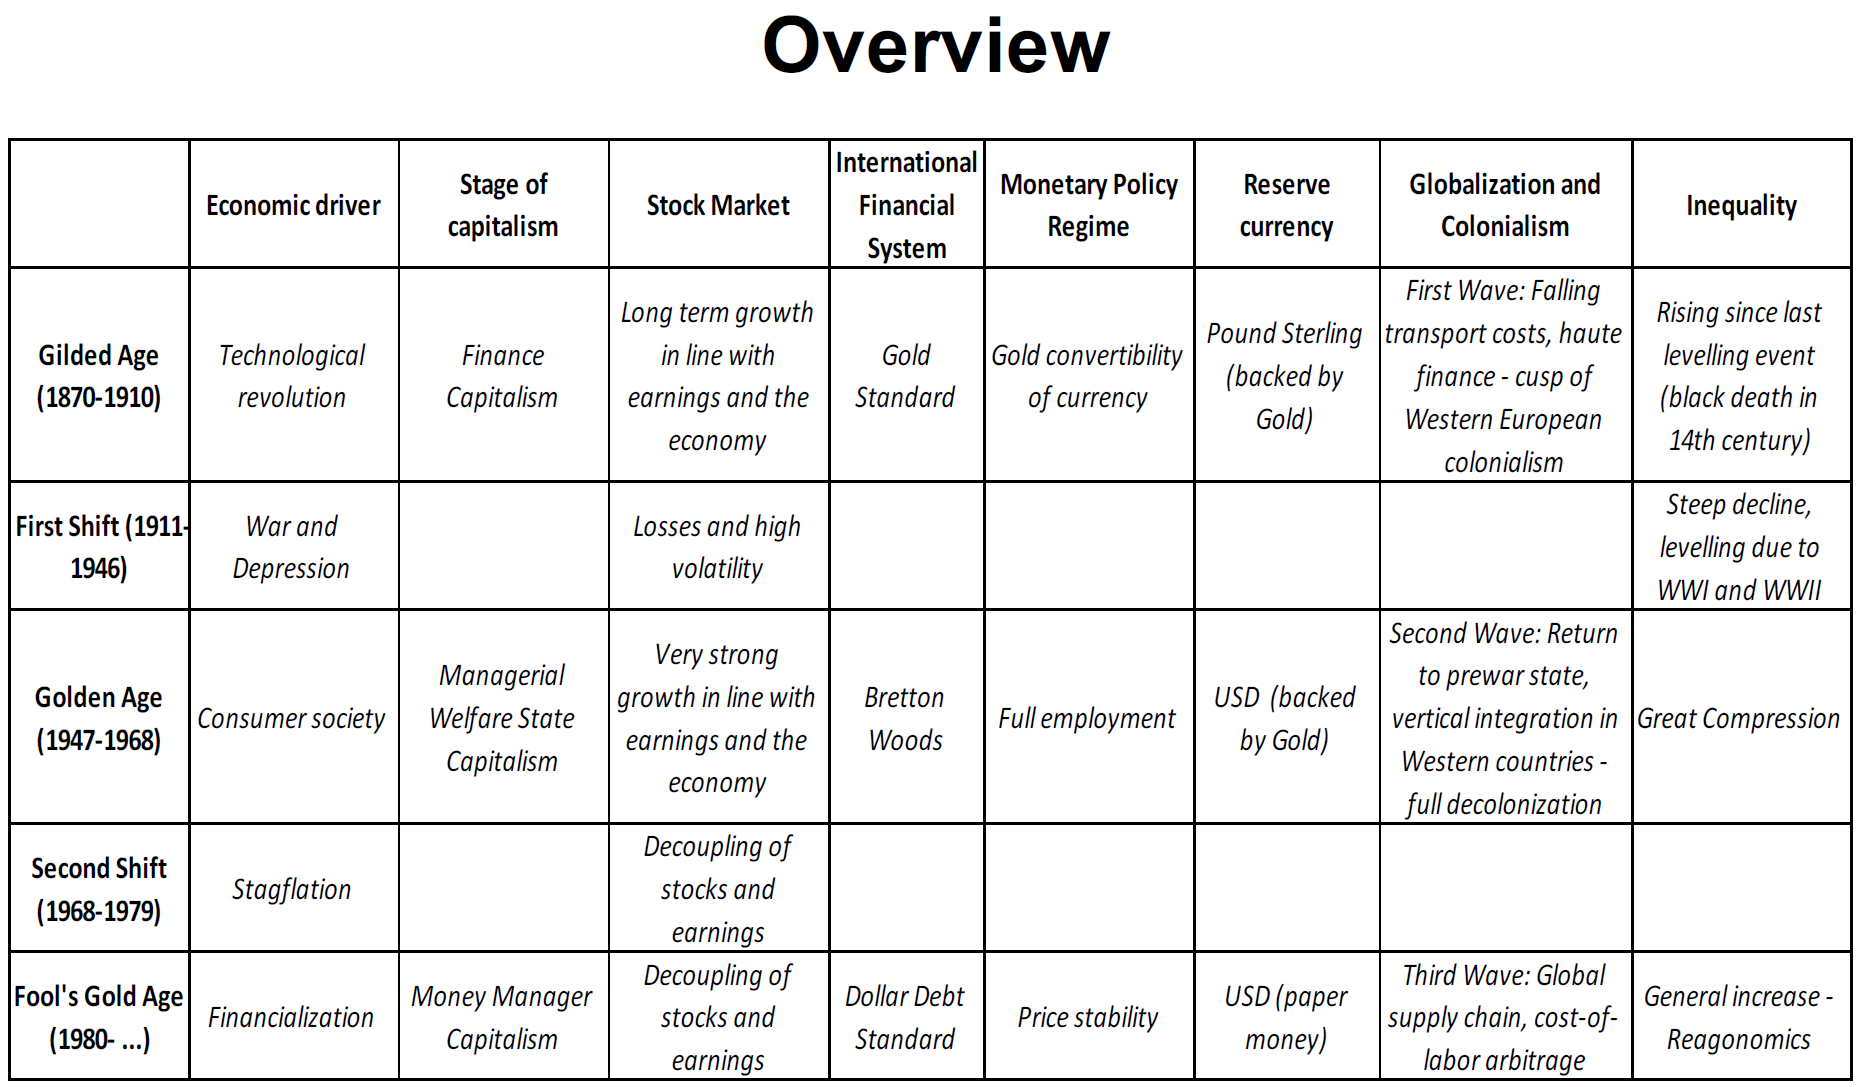
\includegraphics[width=\textwidth]{Pictures/6_Overview.png}
    \caption{Overview}
\end{figure}

\paragraph{A glimpse into the future?}
\begin{itemize}
    \item The Fool's Gold Age has been ongoing for almost three to four
        decades.
    \item I think that around 2008-2019, we have transitioned into a new
        Shift (2020-2050)
    \item The new shift is characterized by many challenges.
\end{itemize}

\paragraph{The future of public debt}
Governments are accumulating debt in an ever-increasing spiral:
\begin{itemize}
    \item GFC (2009)
    \item European Debt crisis (2011)
    \item Covid-19 (2020) and the current multi-trillion stimulus package
\end{itemize}
On top of that there are:
\begin{itemize}
    \item Rising pensions
    \item Healthcare costs
    \item Aging population
\end{itemize}
Towards a new definition of money, direct monetary financing or a debt
jubilee? Chinese DCEP (digital currency electronic payment)

\paragraph{Covid-19 stimulus - how much further can this go?}

\begin{itemize}
    \item \underline{The economist}: At least \$8trn of state loans and
        goodies have been promised to private firms in America and Europe,
        roughly equivalent to al their profits over the past two years. But
        there is still no guarantee that this mountain of money can prevent
        chaos.
    \item \underline{The FT}: Total worldwide stimulus announced since 2020
        comes to about \$14tn, according to the IMF, after adding various
        government spending packages. Such activity has given a big lift
        to asset prices, from stocks to junk bonds.
\end{itemize}

\begin{figure}[h]
    \centering
    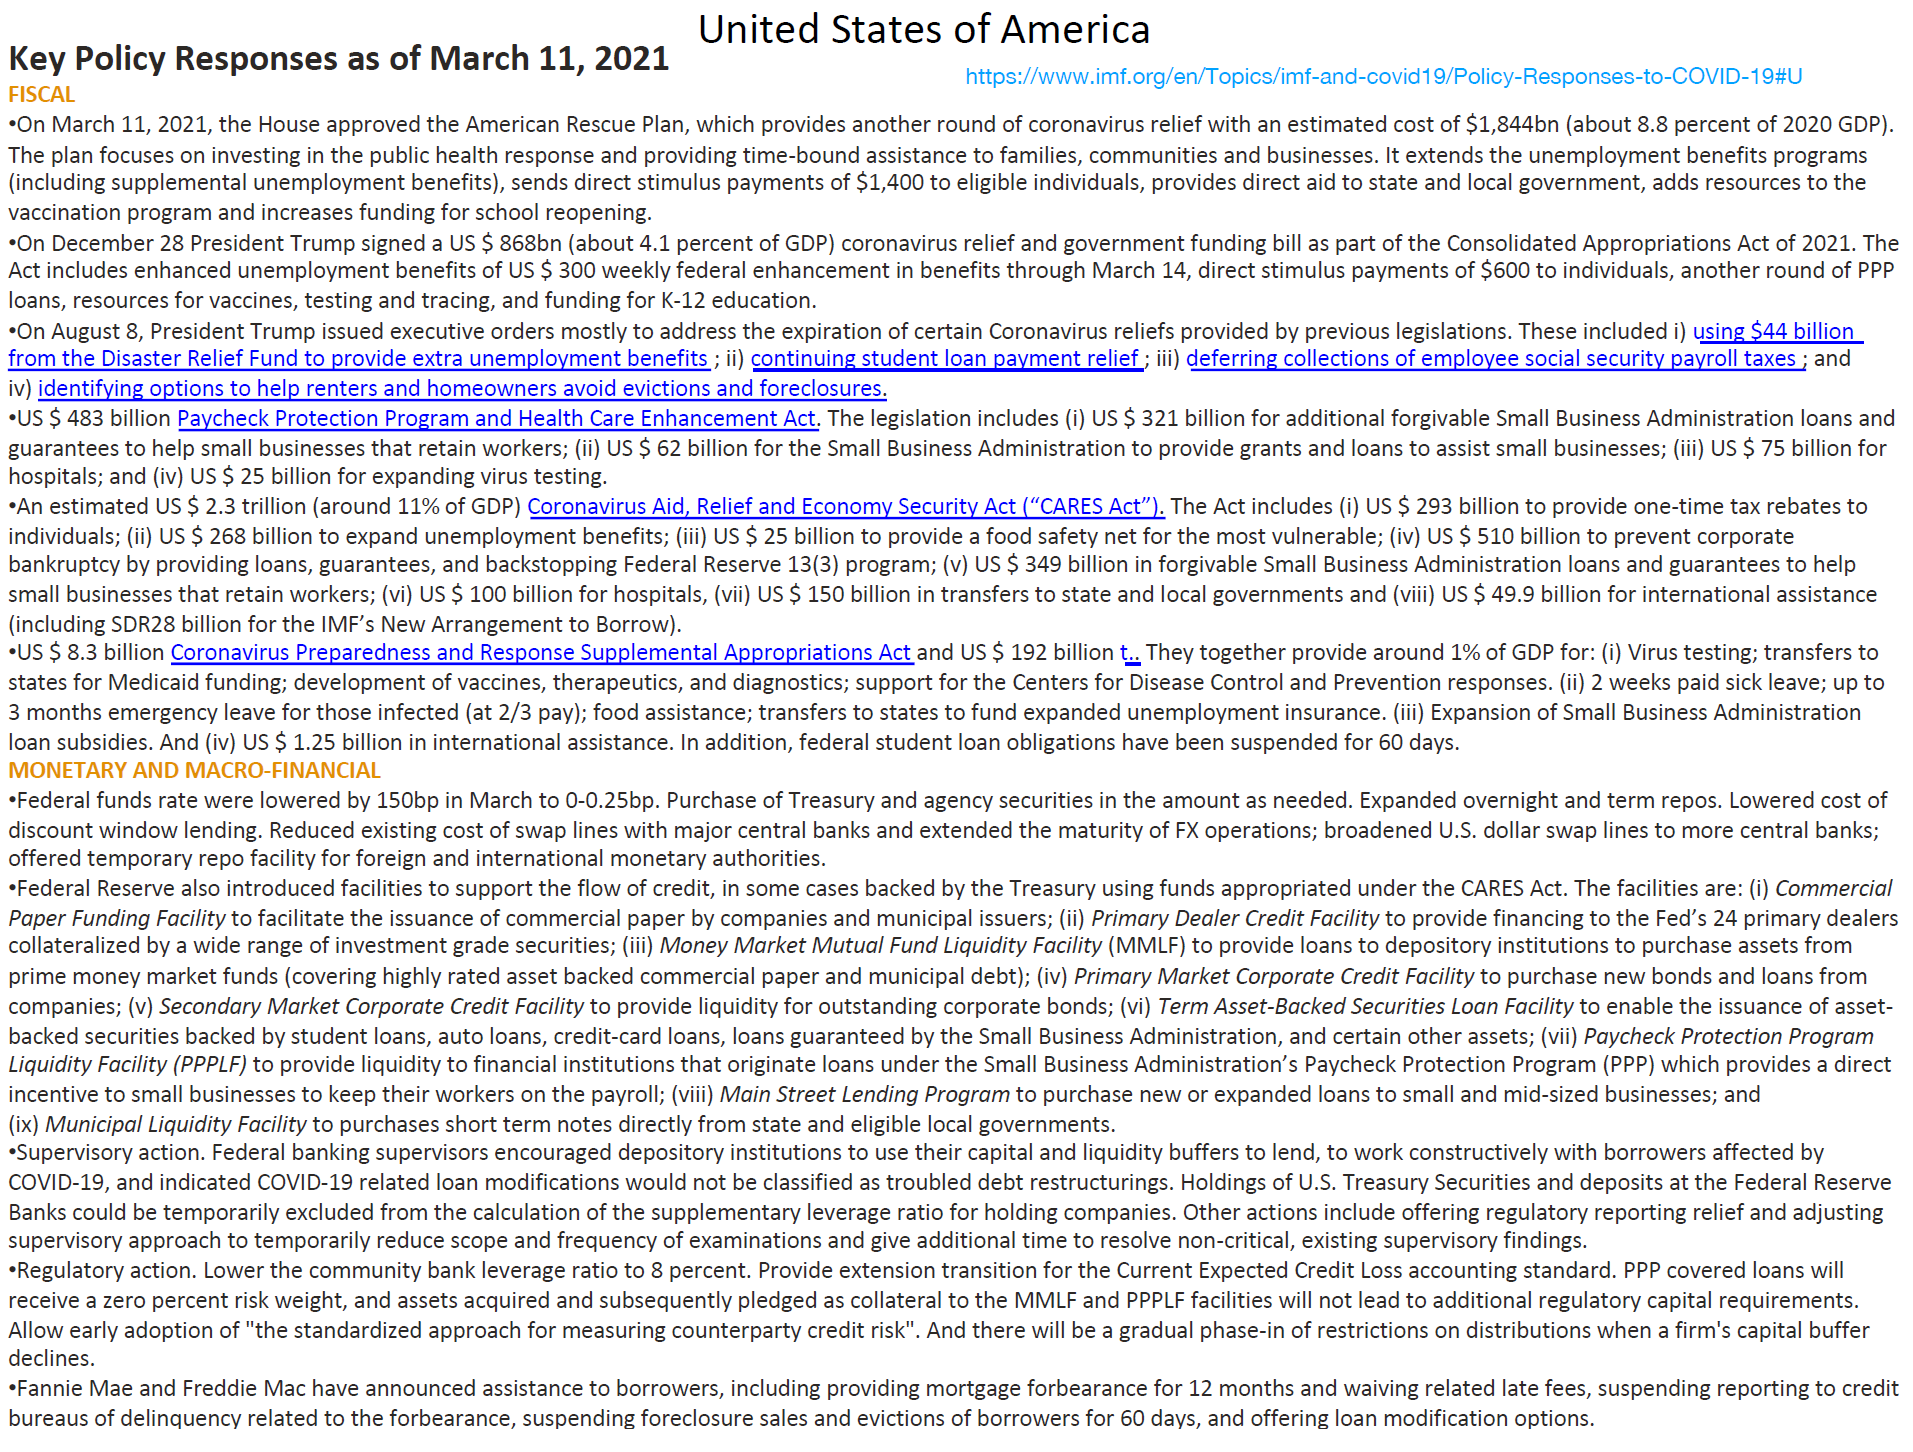
\includegraphics[width=\textwidth]{Pictures/Covid_USA.png}
    \caption{Key policy responses to Civid-19 in the USA}
\end{figure}


\subsubsection{A new bipolar world with two great "empires"?}

With the White House continually provoking tensions against Russia and Chine,
the doyen of American foreign policy, Henry Kissinger, dramatically warned
Washington last week to either agree to a new international system or continue
pushing tensions that are leading to a situation similar to the eve of WW1.

\begin{itemize}
    \item The economy converged with the US at the fastest pace on record.
        China's GDP was $71.4\%$ of US levels in 2020, according to the
        International Monetary Fund, up $4.2\%$ from the previous year
    \item The share of global trade increased as pandemic-related exports
        surged. Already the world's top exporter, China's shipments increased
        $3.6\%$ in 2020, according to official data. Total world trade likely
        contracted $5.6\%$, according to estimates from the United Nations'
        trade and development body UNCTAD
    \item China likely regained the title as the world's top destination for
        foreign investment, which it lost to the US in 2015. Foreign investment
        into China reached more than $\$129.5$ billion through November 2920,
        slightly above the previous year. Globally, FDI flows are likely to have
        fallen $30-40\%$ year-on-year in 2020, according to UNCTAD
    \item The Fortune Global 500 list of the world's largest companies by
        revenue for the first time contained more companies based in China,
        including Hong Kong, than the US: $124$ vs. $121$.
    \item Full-year movie box office receipts overtook the US for the first
        time.
    \item Sovereign debt was added to the FTSE Russel benchmark index,
        completing the country's inclusion in all three top global bond
        indexes. Foreign investors bought $1.1$ trillion yuan (\$ $170$
        billion) of Chinese bonds in 2020.
\end{itemize}

Kishore Mahbubani is a Singaporean civil servant, a career diplomat and an
academic. During his stint at the Ministry of Foreign Affairs from 1971 ot
2004, he served as Singapore's Permanent Representative to the UN and held
the position of President of the UN Security Council between January 2001
and May 2002. Between 2004 and 2017, he served as Dean of the Lee Kuan Yew
School of Public Policy at National University of Singapore.

\vspace{1\baselineskip}

US Army General H.R. McMaster expressed the american attitude succinctly:
"At the end of the day, the struggle between America and China represents
the struggle between 'free and open societies and closed authoritarian
systems.'" And just like the Soviets, the Japanese or the Nazis before them,
this new "authoritarian" challenger, i.e. Chian, barely stands a chance
against America, the de facto torchbearer of Western civilisation.

\vspace{1\baselineskip}

Except this time, as Mahbubani convincingly contends, the choice is not that
straightforward. Burgeoning student debt, housing crisis, an ongoing opioid
epidemic, a poor healthcare system, crumbling infrastructure - these are
tell-tale signs of an empire in decline. Even more striking is the yawning
gap between public policy and public opinion. Mahbubani cites several
credible research papers which document the broad convergence of opinion
among academics that policymaking in US is largely dominated by an increasingly
small economic elite while the average American has little to no say. And
while self-correction is baked into democratic institutions, they to not have
the leeway to make major U-turns in a short timeframe.

\vspace{1\baselineskip}

Big issues: Uighur humanitarian crisis and the Xinjiang separatist movement,
Tibet, Taiwan, Hong Kong, \dots

\paragraph{Pollution, climate change, biodiversity loss}

The big challenge is to develop countries without crossing a sustainability
threshold.

\paragraph{However\dots}

\begin{itemize}
    \item We showed, that regime shifts in society, economy, culture and
        technology are the natural phenomenon.
    \item In the past $150$ years we have seen $2$ shifts and $3$ structural
        regimes.
\end{itemize}

We have seen that revolution, war, depression, genocide, nationalism during
the First Shift let to a response of statesmanship, international cooperation
and fairness (equity):
\begin{itemize}
    \item Institutional reforms (e.g. Roosevelt's New Deal)
    \item International cooperation (e.g. Bretton Woods)
    \item A society contract between owners and workers so that the profits
        of progress are equitably shared
\end{itemize}
How could that happen now? And what could be possible pathways, plans,
changes, solutions?

\paragraph{Project Tellus}

This is what we are trying to achieve with Project Tellus that is being set
up at our chair in cooperation with Risk-X at SUSTech:
"Achieving Human-Earth Sustainability". What is Tellus?
\begin{itemize}
    \item Assemble a broad range of existing visions/insights of how Human-Earth
        Sustainability can be achieved through review of existing research
        and interviews of 'remarkable individuals' (the dragonfly eye view)
    \item Translate these into a systems dynamics model (the Human Earth
        Simulator), whis will serve as a formal repository (of objects and
        interactions linked together in a dynamical system)
    \item Armed with the simulator, generate possible pathways and alternative
        futures that follow our mission, and that can be translated into
        actual and executable plans.
    \item Join forces with stakeholders from industry, policy makers and the
        general public - send out a 'Call for Action', build a cummunity,
        focus on impact and solutions in industry and society.
\end{itemize}

One size does not fit all.

\begin{itemize}
    \item Solutions must look the worldwide socioeconomic system and take
        for real the fact that $85\%$ of the world's inhabitants are trying
        to catch up.
    \item Different regions, with varying economies, political systems and
        cultures need tailored solutions
    \item Carbon emission is only one dimension of humanity's ecological
        footprint. Solving this in isolation is likely to lead to unintended
        consequences. The Human-Earth system faces many more problems like
        biodiversity loss, pollution, health, inequality, stagnating
        economic growth, debt, water scarcity, erosion, waste,\dots
\end{itemize}

We follow these general Principles:

\begin{itemize}
    \item Do not overemphasize the accumulation of knowledge and underemphasize
        the dissemination of what was learned - reach out!
    \item Focus on technical feasibility
    \item Submit any plans and solutions to rigorous simulations
    \item First do no harm ('Primum non nocere'), do not play the sorcer's
        apprentice
    \item Take a worldwide perspective and follow the fox' creed: 'one size
        does not fit all'
    \item Use common sense, prioritize and look foremost for big-impact
        solutions.
\end{itemize}

